\documentclass[letterpaper,10pt]{book}
% Change to 10 pt
\usepackage{pdfpages}
\usepackage{morewrites}			% to counteract the no write space problem
\setcounter{tocdepth}{6}

\usepackage[framemethod=TikZ]{mdframed}

\usepackage{fancyhdr}

\usepackage{paralist}
\usepackage{amsmath}
\usepackage{amsfonts}
\usepackage{amssymb}
\usepackage{graphicx}

\usepackage{datetime}
%\usepackage{ulem}

%\usepackage[nottoc]{toobibind}

\usepackage[inline]{enumitem}

% Outer margin at 2.50 is exacty correct to fit the ``corruption alert'' tables
\usepackage[inner=1.0in, outer=2.50in, top=2.54cm,bottom=2.54cm, marginparwidth=2.25in]{geometry}

\usepackage{marginnote}
\usepackage{longtable}
\usepackage{booktabs}
\usepackage{xcolor}

\usepackage{soul}

%%%%%%%%%%%%
\definecolor{ForestGreen}{rgb}{0.00,0.29,0.098}
%%%%%%%%%%%%

\usepackage{marginnote}

\usepackage{imakeidx} 
\usepackage[
	backref=true,
	style=numeric,
%	citestyle=numeric,
	backend=bibtex
	]{biblatex}
\usepackage[driverfallback=hypertex,colorlinks=True]{hyperref}
\usepackage{cleveref}

\makeindex[name=scripture,columnsep=20pt, columnseprule=True,columns=3, title=Scripture References]
\makeindex[name=speaker,columnsep=20pt, columnseprule=True,,columns=2, title=Sermon Creator]
\makeindex[name=series,columnsep=20pt, columnseprule=True,,columns=2, title=Sermon Series]
\makeindex[name=date,columnsep=20pt, columnseprule=True,columns=2, title=Sermon Date]
\makeindex[name=event,columnsep=20pt, columnseprule=True,columns=2, title=Event]
\makeindex[name=topic,columnsep=20pt, columnseprule=True,columns=2, title=Topic]
\makeindex[name=AWIP,columnsep=20pt, columnseprule=True,columns=3, title=All Words in Passage]
\makeindex[name=NWIV,columnsep=20pt, columnseprule=True,columns=3, title=Number of Words in Verse]
\makeindex[name=PNIP,columnsep=20pt, columnseprule=True,columns=3, title=Proper Names in Passage]
\makeindex[name=PEIP,columnsep=20pt, columnseprule=True,columns=2, title=Prophetic Events in Passage]
\makeindex[name=TWPAQ,columnsep=20pt, columnseprule=True,columns=1, title=13-Word Phrases and Quotes]
\makeindex[name=PFTTIS,columnsep=20pt, columnseprule=False,columns=3, title=Phrases found 13 times in scripture]
\makeindex[name=WFTTIS,columnsep=20pt, columnseprule=False,columns=3, title=Words found 13 times in scripture]
\makeindex[name=WFITV,columnsep=20pt, columnseprule=False,columns=3, title=Words found in exactly 13 verses]
\makeindex[name=EVENTS,columnsep=20pt, columnseprule=False,columns=2, title=Sermon Log by Place]
\makeindex[name=QUESTIONS,columnsep=20pt, columnseprule=False,columns=2, title=Bible Questions]
\makeindex[name=DOCTRINES,columnsep=20pt, columnseprule=False,columns=2, title=Doctrines]
\makeindex[name=SONGS,columnsep=20pt, columnseprule=False,columns=1, title=Songs]
\makeindex[name=LOCATION,columnsep=20pt, columnseprule=False,columns= 2, title=Location]
\makeindex[name=FACEBOOK,columnsep=20pt, columnseprule=False,columns=2, title=Facebook]
\makeindex[name=DEVOTIONAL,columnsep=20pt, columnseprule=False,columns=2, title=Devotional Items]
%%%%%%%%%%%%%%%%% EXTRA COLORS
\definecolor{champagne}{rgb}{0.97,0.91,0.81}
\definecolor{bone}{rgb}{0.89,0.85,0.79}
\pagestyle{fancy}
\fancyhf{}
\fancyhead[LE,RO]{\today}
\fancyhead[RE,LO]{Daily Bible Reading}
\fancyhead[CE,CO]{-page \thepage  - }

\fancyfoot[CO,CE]{\leftmark}
%\fancyfoot[LE,RO]{CSCE 692, HW1}

\title{DBR\\
Daily \\ Reads}
\author{Keith Anthony \\
\today }
%+/ffffff +   \pagenumbering{gobble}
\bibliography{Bibliographies/All20220122}

\setlength{\fboxsep}{1.0pt}

\usepackage[utf8]{inputenc}
\usepackage{tikz}

\begin{document}
%%%%%%%%%%%% Tile Page

\begin{titlepage}

\begin{flushright}
\rightskip=-2.5cm
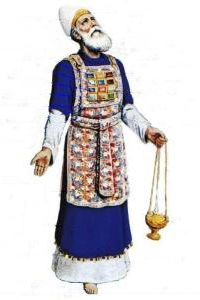
\includegraphics[width=50mm,scale=1.5]{Extras/Melchisedec.jpg}
\vspace{0.4in}  % Create a title for the document and write it in bold font
\LARGE{\textbf{\date}} % Again, do a line break
\linebreak 
% Create a subtitle \large{with Outlines, Statistics, Cross References, and Notes}
\vspace{0.5in}
\begin{flushleft}
\LARGE{Day \#73: Tuesday, 15  March 2022 PLAIN  \\}\vspace{0.25in}
\LARGE{Judges 4-6 Psalm 74 Proverb 15}
\end{flushleft}
\vspace{0.6in}
\bigskip

\normalsize{Xenia, Oh.\\}
\normalsize{created: \today}
\vspace{1.3in}

\end{flushright}
\end{titlepage}

\newpage 
\tableofcontents\hypertarget{TOC}{}
\listoffigures
\listoftables

\hyphenation{A-bim-e-lech bre-thren E-phra-im  Gib-e-o-nites Jer-u-sa-lem through-out Phil-i-stines The-o-phil-us Am-a-le-kites ven-geance Mesh-el-e-mi-ah onan-ism Phar-a-oh thoughts grev-ous-ness Hach-a-liah adul-ter-er Shad-rach}

%%%%%%%%%%%%%%%%% EXTRA COLORS
%%%%%%%%%%%%%%%%% EXTRA COLORS
%%%%%%%%%%%%%%%%% EXTRA COLORS
\definecolor{champagne}{rgb}{0.97,0.91,0.81}
\definecolor{bone}{rgb}{0.89,0.85,0.79}

\definecolor{ForestGreen}{rgb}{0.00,0.29,0.098}
\definecolor{GIVING}{cmyk}{1,0.0,0.72,.1}

\definecolor{MLPE}{cmyk}{1,1,0,.45}
\definecolor{SOCCER}{cmyk}{.77, 0, .42, .49}
\definecolor{PAYBILL}{cmyk}{0,0.83,0.76,0.07}
\definecolor{SERMON}{cmyk}{.14,.9,0,.30} % aka seance \href{http://www.flatuicolorpicker.com/purple-cmyk-color-model/}{seance}
\definecolor{BIBLE}{cmyk}{0,.17,.74,.17}
\definecolor{WORKBLUE}{cmyk}{1, .5, 0, .6}
\definecolor{myOrange}{cmyk}{0, .4, .98, .03}
\definecolor{myTan}{cmyk}{0.0,.07,.17,.10}
\definecolor{myRed}{cmyk}{0,1,1,0}
\definecolor{myWhite}{cmyk}{0,0,0,0}
\definecolor{BLUESoD}{cmyk}{.97,.84,0,.04}
\definecolor{WHITE}{cmyk}{0,0,0,0}
\definecolor{OLDGOLD}{cmyk}{0.05,0.3,1.00,0}
\definecolor{CASTLETON}{cmyk}{1,0,0.31,0.66}
\definecolor{cadmiumgreen}{rgb}{0.0, 0.42, 0.24}
\definecolor{jungle}{rgb}{0.203,0.4882,0.1718}
\definecolor{MYGOLD}{rgb}{1,.84,0}

\definecolor{MYLIGHTGRAY}{rgb}{.85,.85,.85}

\definecolor{codegreen}{rgb}{0,0.6,0}
\definecolor{codegray}{rgb}{0.5,0.5,0.5}
\definecolor{codepurple}{rgb}{0.58,0,0.82}
\definecolor{backcolour}{rgb}{0.95,0.95,0.92}


\mdfdefinestyle{MyFrame}{%
    linecolor=blue,
    outerlinewidth=2pt,
    roundcorner=5pt,
    innertopmargin=\baselineskip,
    innerbottommargin=\baselineskip,
    innerrightmargin=10pt,
    innerleftmargin=10pt,
    backgroundcolor=gray!25!white}


\mdfdefinestyle{MyFrame2}{%
    linecolor=black,
    outerlinewidth=2pt,
    roundcorner=5pt,
    innertopmargin=\baselineskip,
    innerbottommargin=\baselineskip,
    innerrightmargin=10pt,
    innerleftmargin=10pt,
    backgroundcolor=yellow!25!white}


%%%%%
%% for PFTTIS list
%%%%%

%%% And Joseph said unto
\index[PFTTIS]{And Joseph said unto!Genesis!Gen 40:008}
\index[PFTTIS]{And Joseph said unto!Genesis!Gen 40:012}
\index[PFTTIS]{And Joseph said unto!Genesis!Gen 41:025}
\index[PFTTIS]{And Joseph said unto!Genesis!Gen 42:014}
\index[PFTTIS]{And Joseph said unto!Genesis!Gen 42:018}
\index[PFTTIS]{And Joseph said unto!Genesis!Gen 44:015}
\index[PFTTIS]{And Joseph said unto!Genesis!Gen 45:003}
\index[PFTTIS]{And Joseph said unto!Genesis!Gen 45:004}
\index[PFTTIS]{And Joseph said unto!Genesis!Gen 46:031}
\index[PFTTIS]{And Joseph said unto!Genesis!Gen 48:009}
\index[PFTTIS]{And Joseph said unto!Genesis!Gen 48:018}
\index[PFTTIS]{And Joseph said unto!Genesis!Gen 50:019}
\index[PFTTIS]{And Joseph said unto!Genesis!Gen 50:024}


%%% a shadow
\index[PFTTIS]{a shadow!1Chronicles!1Chr 029:15}
\index[PFTTIS]{a shadow!Job!Job 008:09}
\index[PFTTIS]{a shadow!Job!Job 014:02}
\index[PFTTIS]{a shadow!Job!Job 017:07}
\index[PFTTIS]{a shadow!Psalm!Psa 102:011}
\index[PFTTIS]{a shadow!Psalm!Psa 144:004}
\index[PFTTIS]{a shadow!Ecclesiastes!Eccl 006:012}
\index[PFTTIS]{a shadow!Ecclesiastes!Eccl 008:013}
\index[PFTTIS]{a shadow!Isaiah!Isa 04:006}
\index[PFTTIS]{a shadow!Isaiah!Isa 25:004}
\index[PFTTIS]{a shadow!Jonah!Jnh 04:06}
\index[PFTTIS]{a shadow!Colossians!Col 02:017}
\index[PFTTIS]{a shadow!Hebews!Heb 10:001}

%%% blessed is the man
\index[PFTTIS]{blessed is the man!Psalm!Psa 001:001}
\index[PFTTIS]{blessed is the man!Psalm!Psa 032:002}
\index[PFTTIS]{blessed is the man!Psalm!Psa 034:008}
\index[PFTTIS]{blessed is the man!Psalm!Psa 065:004}
\index[PFTTIS]{blessed is the man!Psalm!Psa 084:005}
\index[PFTTIS]{blessed is the man!Psalm!Psa 084:012}
\index[PFTTIS]{blessed is the man!Psalm!Psa 094:012}
\index[PFTTIS]{blessed is the man!Psalm!Psa 112:001}
\index[PFTTIS]{blessed is the man!Proverbs!Pro 008:034}
\index[PFTTIS]{blessed is the man!Isaiah!Isa 056:002}
\index[PFTTIS]{blessed is the man!Jeremiah!Jer 017:007}
\index[PFTTIS]{blessed is the man!Romans!Rom 004:008}
\index[PFTTIS]{blessed is the man!James!Jam 001:012}


%%% carry them
\index[PFTTIS]{carry them!Leviticus!Lev 14:045}
\index[PFTTIS]{carry them!Numbers!Num 11:012}
\index[PFTTIS]{carry them!Joshua!Jsh 04:003}
\index[PFTTIS]{carry them!1Samuel!1Sam 20:040}
\index[PFTTIS]{carry them!1Kings!1Kng 08:046}
\index[PFTTIS]{carry them!2Chronicles!2Chr 06:036}
\index[PFTTIS]{carry them!Ezra!Ezra 05:015}
\index[PFTTIS]{carry them!Isaiah!Isa 40:011}
\index[PFTTIS]{carry them!Isaiah!Isa 41:016}
\index[PFTTIS]{carry them!Isaiah!Isa 57:013}
\index[PFTTIS]{carry them!Jeremiah!Jer 20:004}
\index[PFTTIS]{carry them!Jeremiah!Jer 20:005}
\index[PFTTIS]{carry them!Jeremiah!Jer 43:012}


\index[PFTTIS]{good tidings!2Samuel!2Sam 18:027}
\index[PFTTIS]{good tidings!1Kings!1Ki 01:042}
\index[PFTTIS]{good tidings!2Kings!2Ki 07:009 (2x)}
\index[PFTTIS]{good tidings!Isaiah!Isa 40:009 (2x)}
\index[PFTTIS]{good tidings!Isaiah!Isa 41:007}
\index[PFTTIS]{good tidings!Isaiah!Isa 52:007}
\index[PFTTIS]{good tidings!Isaiah!Isa 61:001}
\index[PFTTIS]{good tidings!Nahum!Nah 01:005}
\index[PFTTIS]{good tidings!Luke!Lk 02:010}
\index[PFTTIS]{good tidings!1Thessalonians!1Thess 03:006}


%%% dead body
\index[PFTTIS]{dead body!Leviticus!Lev 21:011}
\index[PFTTIS]{dead body!Numbers!Num 06:006}
\index[PFTTIS]{dead body!Numbers!Num 09:006}
\index[PFTTIS]{dead body!Numbers!Num 09:007}
\index[PFTTIS]{dead body!Numbers!Num 09:010}
\index[PFTTIS]{dead body!Numbers!Num 09:011}
\index[PFTTIS]{dead body!Numbers!Num 09:013}
\index[PFTTIS]{dead body!Numbers!Num 09:016}
\index[PFTTIS]{dead body!2Kings!2Ki 08:005}
\index[PFTTIS]{dead body!Isaiah!Isa 26:019}
\index[PFTTIS]{dead body!Jeremiah!Jer 26:023}
\index[PFTTIS]{dead body!Jeremiah!Jer 36:030}
\index[PFTTIS]{dead body!Haggai!Hag 02:013}

%%% great sea
\index[PFTTIS]{great sea!Numbers!Num 34:006}
\index[PFTTIS]{great sea!Numbers!Num 34:007}
\index[PFTTIS]{great sea!Joshua!Jos 01:004}
\index[PFTTIS]{great sea!Joshua!Jos 09:001}
\index[PFTTIS]{great sea!Joshua!Jos 15:012}
\index[PFTTIS]{great sea!Joshua!Jos 15:047}
\index[PFTTIS]{great sea!Joshua!Jos 23:004}
\index[PFTTIS]{great sea!Ezekiel!Eze 47:010}
\index[PFTTIS]{great sea!Ezekiel!Eze 47:015}
\index[PFTTIS]{great sea!Ezekiel!Eze 47:019}
\index[PFTTIS]{great sea!Ezekiel!Eze 47:020}
\index[PFTTIS]{great sea!Ezekiel!Eze 48:028}
\index[PFTTIS]{great sea!Daniel!Dan 07:002}


%%% have forsaken me
\index[PFTTIS]{have forsaken me!Judges!Jdg 10:013}
\index[PFTTIS]{have forsaken me!1Samuel!1Sam 08:008}
\index[PFTTIS]{have forsaken me!1Kings!1Ki 11:033}
\index[PFTTIS]{have forsaken me!2Kings!2Ki 22:017}
\index[PFTTIS]{have forsaken me!2Chronicles!2Chr 12:005}
\index[PFTTIS]{have forsaken me!2Chronicles!2Chr 34:025}
\index[PFTTIS]{have forsaken me!Jeremiah!Jer 01:016}
\index[PFTTIS]{have forsaken me!Jeremiah!Jer 02:013}
\index[PFTTIS]{have forsaken me!Jeremiah!Jer 05:007}
\index[PFTTIS]{have forsaken me!Jeremiah!Jer 05:019}
\index[PFTTIS]{have forsaken me!Jeremiah!Jer 16:011 (2x)}
\index[PFTTIS]{have forsaken me!Jeremiah!Jer 19:004}

%%% no king
\index[PFTTIS]{no king!Judges!Jdg 17:06}
\index[PFTTIS]{no king!Judges!Jdg 18:01}
\index[PFTTIS]{no king!Judges!Jdg 19:01}
\index[PFTTIS]{no king!Judges!Jdg 21:25}
\index[PFTTIS]{no king!1Kings!1Ki 22:47}
\index[PFTTIS]{no king!2Kings!2Ki 23:25}
\index[PFTTIS]{no king!Nehemiah!Neh 13:26}
\index[PFTTIS]{no king!Psalms!Psa 033:016}
\index[PFTTIS]{no king!Proverbs!Pro 30:27}
\index[PFTTIS]{no king!Daniel!Dan 02:10}
\index[PFTTIS]{no king!Hosea!Hos 10:03}
\index[PFTTIS]{no king!Micah!Mic 04:09}
\index[PFTTIS]{no king!John!Jhn 19:15}


%%% rebellious house
\index[PFTTIS]{rebellious house!Exodus!Exo 02:005}
\index[PFTTIS]{rebellious house!Exodus!Exo 02:006}
\index[PFTTIS]{rebellious house!Exodus!Exo 02:008}
\index[PFTTIS]{rebellious house!Exodus!Exo 03:009}
\index[PFTTIS]{rebellious house!Exodus!Exo 03:026}
\index[PFTTIS]{rebellious house!Exodus!Exo 03:027}
\index[PFTTIS]{rebellious house!Exodus!Exo 12:002 (2x)}
\index[PFTTIS]{rebellious house!Exodus!Exo 12:003}
\index[PFTTIS]{rebellious house!Exodus!Exo 12:009}
\index[PFTTIS]{rebellious house!Exodus!Exo 12:025}
\index[PFTTIS]{rebellious house!Exodus!Exo 17:012}
\index[PFTTIS]{rebellious house!Exodus!Exo 24:003}

%%% seek him
\index[PFTTIS]{seek him!Deuteronomy!Deu 04:029}\index[PFTTIS]{seek him!1Samuel!1Sam 23:025}
\index[PFTTIS]{seek him!1Chronicles!1Chr 28:009}
\index[PFTTIS]{seek him!2Chronicles!1Chr 15:002}
\index[PFTTIS]{seek him!Ezra!Ezr 08:022}
\index[PFTTIS]{seek him!Psalms!Psa 022:026}
\index[PFTTIS]{seek him!Psalms!Psa 024:006}
\index[PFTTIS]{seek him!Psalms!Psa 119:002}
\index[PFTTIS]{seek him!SoS!SoS 03:002}
\index[PFTTIS]{seek him!SoS!SoS 06:001}
\index[PFTTIS]{seek him!Hosea!Hos 07:010}
\index[PFTTIS]{seek him!Amos!Amo 05:008}
\index[PFTTIS]{seek him!Hebrews!Heb 11:0063}


%%% seek ye
\index[PFTTIS]{seek ye!Isaiah!Isa 34:016}
\index[PFTTIS]{seek ye!Isaiah!Isa 45:019}
\index[PFTTIS]{seek ye!Isaiah!Isa 55:006}
\index[PFTTIS]{seek ye!Amos!Amos 5:004}
\index[PFTTIS]{seek ye!John!John 1:38}
\index[PFTTIS]{seek ye!John!John 18:4}
\index[PFTTIS]{seek ye!John!John 18:7}
\index[PFTTIS]{seek ye!Matthew!Matt 6:33}
\index[PFTTIS]{seek ye!Numbers!Num 16:10}
\index[PFTTIS]{seek ye!Luke!Luke 12:31}
\index[PFTTIS]{seek ye!Luke!Luke 24:5}
\index[PFTTIS]{seek ye!Psalm!Psa 27:8}
\index[PFTTIS]{seek ye!Zephaniah!Zeph 2:3}

%%% the uncircumcised
\index[PFTTIS]{the uncircumcised!Genesis!Gen 17:014}
\index[PFTTIS]{the uncircumcised!Judges!Jdg 14:003}
\index[PFTTIS]{the uncircumcised!Judges!Jdg 15:018}
\index[PFTTIS]{the uncircumcised!2Samuel!2Sam 01:020}
\index[PFTTIS]{the uncircumcised!Isaiah!Isa 02:001}
\index[PFTTIS]{the uncircumcised!Jeremiah!Jer 09:025}
\index[PFTTIS]{the uncircumcised!Ezekiel!Eze 28:010}
\index[PFTTIS]{the uncircumcised!Ezekiel!Eze 31:018}
\index[PFTTIS]{the uncircumcised!Ezekiel!Eze 32:019}
\index[PFTTIS]{the uncircumcised!Ezekiel!Eze 32:027}
\index[PFTTIS]{the uncircumcised!Ezekiel!Eze 32:028}
\index[PFTTIS]{the uncircumcised!Ezekiel!Eze 32:029}
\index[PFTTIS]{the uncircumcised!Ezekiel!Eze 32:032}

%%% worship him
\index[PFTTIS]{worship him!Psalms!Psa 97:007}
\index[PFTTIS]{worship him!Zephaniah!Zeph 02:011}
\index[PFTTIS]{worship him!Matthew!Matt 02:002}
\index[PFTTIS]{worship him!Matthew!Matt 02:008}
\index[PFTTIS]{worship him!John!John 04:023}
\index[PFTTIS]{worship him!John!John 04:024 (2x)} 
\index[PFTTIS]{worship him!Acts!Acts 17:023}
\index[PFTTIS]{worship him!Hebrews!Heb 01:006}
\index[PFTTIS]{worship him!Revelation!Rev 04:010}
\index[PFTTIS]{worship him!Revelation!Rev 13:008}
\index[PFTTIS]{worship him!Revelation!Rev 14:007}
\index[PFTTIS]{worship him!Revelation!Rev 19:010}


%%%%%
%% for PFTTIS list
%%%%%

%%% afflictions
\index[WFTTIS]{afflictions!Psalms!Psa 34:019}
\index[WFTTIS]{afflictions!Psalms!Psa 132:001}
\index[WFTTIS]{afflictions!Acts!Acts 07:010}
\index[WFTTIS]{afflictions!Acts!Acts 20:023}
\index[WFTTIS]{afflictions!2Corinthians!2Cor 06:004}
\index[WFTTIS]{afflictions!Colossians!Col 01:024}
\index[WFTTIS]{afflictions!1Thessalonians!1Thess 03:003}
\index[WFTTIS]{afflictions!2Timothy!2Tim 01:008}
\index[WFTTIS]{afflictions!2Timothy!2Tim 03:011}
\index[WFTTIS]{afflictions!2Timothy!2Tim 04:005}
\index[WFTTIS]{afflictions!Hebrews!Heb 10:032}
\index[WFTTIS]{afflictions!Hebrews!Heb 10:033}
\index[WFTTIS]{afflictions!1Peter!1Pet 05:009}

%%% acsend
\index[WFTTIS]{acsend!Joshua!Jos 06:05}
\index[WFTTIS]{acsend!Psalm!Psa 024:003}
\index[WFTTIS]{acsend!Psalm!Psa 135:007}
\index[WFTTIS]{acsend!Psalm!Psa 139:008}
\index[WFTTIS]{acsend!Isaiah!Isa 14:013}
\index[WFTTIS]{acsend!Isaiah!Isa 14:014}
\index[WFTTIS]{acsend!Jeremiah!Jer 10:013}
\index[WFTTIS]{acsend!Jeremiah!Jer 51:016}
\index[WFTTIS]{acsend!Ezekiel!Eze 38:009}
\index[WFTTIS]{acsend!John!John 06:062}
\index[WFTTIS]{acsend!John!John 20:017}
\index[WFTTIS]{acsend!Romans!Rom 10:006}
\index[WFTTIS]{acsend!Revelation!Rev 17:008}

%%% Assyrian
\index[WFTTIS]{Assyrian!Isaiah!Isa 10:005}
\index[WFTTIS]{Assyrian!Isaiah!Isa 10:024}
\index[WFTTIS]{Assyrian!Isaiah!Isa 14:025}
\index[WFTTIS]{Assyrian!Isaiah!Isa 19:023}
\index[WFTTIS]{Assyrian!Isaiah!Isa 23:013}
\index[WFTTIS]{Assyrian!Isaiah!Isa 30:031}
\index[WFTTIS]{Assyrian!Isaiah!Isa 31:008}
\index[WFTTIS]{Assyrian!Isaiah!Isa 52:004}
\index[WFTTIS]{Assyrian!Ezekiel!Eze 31:003}
\index[WFTTIS]{Assyrian!Hosea!Hos 05:013}
\index[WFTTIS]{Assyrian!Hosea!Hos 11:005}
\index[WFTTIS]{Assyrian!Micah!Hos 05:005}
\index[WFTTIS]{Assyrian!Micah!Hos 05:006}

%%% blot
\index[WFTTIS]{blot!Exodus!Exo 32:032}
\index[WFTTIS]{blot!Exodus!Exo 32:033}
\index[WFTTIS]{blot!Numbers!Num 05:026}
\index[WFTTIS]{blot!Deuteronomy!Deut 09:014}
\index[WFTTIS]{blot!Deuteronomy!Deut 25:019}
\index[WFTTIS]{blot!Deuteronomy!Deut 29:020}
\index[WFTTIS]{blot!2Kings!2Ki 14:027}
\index[WFTTIS]{blot!Job!Job 31:007}
\index[WFTTIS]{blot!Psalms!Psa 51:001}
\index[WFTTIS]{blot!Psalms!Psa 51:009}
\index[WFTTIS]{blot!Proverbs!Pro 09:007}
\index[WFTTIS]{blot!Jeremiah!Jer 18:023}
\index[WFTTIS]{blot!Revelation!Rev 03:005}


%%% chain
\index[WFTTIS]{chain!Genesis!Gen 41:042}
\index[WFTTIS]{chain!1Kings!1Ki 07:017}
\index[WFTTIS]{chain!Psalms!Psa 73:006}
\index[WFTTIS]{chain!SoS!Sos 04:009}
\index[WFTTIS]{chain!Lamentations!Lam 03:007}
\index[WFTTIS]{chain!Ezekiel!Eze 07:023}
\index[WFTTIS]{chain!Ezekiel!Eze 16:011}
\index[WFTTIS]{chain!Daniel!Dan 05:007}
\index[WFTTIS]{chain!Daniel!Dan 05:016}
\index[WFTTIS]{chain!Daniel!Dan 05:029}
\index[WFTTIS]{chain!Acts!Acts 28:020}
\index[WFTTIS]{chain!2Timothy!2Tim 01:016}
\index[WFTTIS]{chain!Revelation!Rev 20:001}


%%% controversy
\index[WFTTIS]{controversy!Deuteronomy!Deu 17:008}
\index[WFTTIS]{controversy!Deuteronomy!Deu 19:017}
\index[WFTTIS]{controversy!Deuteronomy!Deu 21:005}
\index[WFTTIS]{controversy!Deuteronomy!Deu 25:001}
\index[WFTTIS]{controversy!2Samuel!2Sam 15:002}
\index[WFTTIS]{controversy!Isaiah!Isa 34:008}
\index[WFTTIS]{controversy!Jeremiah!Jer 25:031}
\index[WFTTIS]{controversy!Ezekiel!Eze 44:024}
\index[WFTTIS]{controversy!Hosea!Hos 04:001}
\index[WFTTIS]{controversy!Hosea!Hos 12:002}
\index[WFTTIS]{controversy!Micah!Mic 06:002 (2x)}
\index[WFTTIS]{controversy!1Timothy!1Tim 03:016}


%%% Dagon/Dagon's
\index[WFTTIS]{Dagon!Judges!Jdg 16:023}
\index[WFTTIS]{Dagon!1Samuel!1Sam 05:002 (2x)}
\index[WFTTIS]{Dagon!1Samuel!1Sam 05:003 (2x)}
\index[WFTTIS]{Dagon!1Samuel!1Sam 05:004 (3x)}
\index[WFTTIS]{Dagon!1Samuel!1Sam 05:005 (3x)}
\index[WFTTIS]{Dagon!1Samuel!1Sam 05:007}
\index[WFTTIS]{Dagon!1Chronicles!1Chr 10:010}

%%% disobedient
\index[WFTTIS]{disobedient!1Kings!1Ki 13:026}
\index[WFTTIS]{disobedient!Nehemiah!Neh 09:026}
\index[WFTTIS]{disobedient!Luke!Luke 01:017}
\index[WFTTIS]{disobedient!Acts!Acts 26:019}
\index[WFTTIS]{disobedient!Romans!Rom 01:030}
\index[WFTTIS]{disobedient!Romans!Rom 10:021}
\index[WFTTIS]{disobedient!1Timothy!1Tim 01:009}
\index[WFTTIS]{disobedient!2Timothy!2Tim 03:002}
\index[WFTTIS]{disobedient!Titus!Titus 01:016}
\index[WFTTIS]{disobedient!Titus!Titus 03:003}
\index[WFTTIS]{disobedient!1Peter!1Pet 02:007}
\index[WFTTIS]{disobedient!1Peter!1Pet 02:008}
\index[WFTTIS]{disobedient!1Peter!1Pet 03:020}


%%% doubt
\index[WFTTIS]{doubt!Genesis!Gen 37:033}
\index[WFTTIS]{doubt!Deuteronomy!Deu 28:066}
\index[WFTTIS]{doubt!Job!Job 12:002}
\index[WFTTIS]{doubt!Matthew!Matt 14:031}
\index[WFTTIS]{doubt!Matthew!Matt 21:021}
\index[WFTTIS]{doubt!Mark!Mk 11:023}
\index[WFTTIS]{doubt!Luke!Lk 11:020}
\index[WFTTIS]{doubt!John!Jhn 10:024}
\index[WFTTIS]{doubt!Acts!Acts 02:012}
\index[WFTTIS]{doubt!Acts!Acts 28:004}
\index[WFTTIS]{doubt!1Corinthians!1Cor 09:010}
\index[WFTTIS]{doubt!Galatians!Gal 04:020}
\index[WFTTIS]{doubt!1John!1Jhn 02:019}


%%% dungeon
\index[WFTTIS]{dungeon!Genesis!Gen 40:015}
\index[WFTTIS]{dungeon!Genesis!Gen 41:014}
\index[WFTTIS]{dungeon!Exodus!Exo 12:029}
\index[WFTTIS]{dungeon!Jeremiah!Jer 37:016}
\index[WFTTIS]{dungeon!Jeremiah!Jer 38:006 (2x)}
\index[WFTTIS]{dungeon!Jeremiah!Jer 38:007}
\index[WFTTIS]{dungeon!Jeremiah!Jer 38:009}
\index[WFTTIS]{dungeon!Jeremiah!Jer 38:010}
\index[WFTTIS]{dungeon!Jeremiah!Jer 38:011}
\index[WFTTIS]{dungeon!Jeremiah!Jer 38:013}
\index[WFTTIS]{dungeon!Lamentations!Lam 03:053}
\index[WFTTIS]{dungeon!Lamentations!Lam 03:055}


%%% error
\index[WFTTIS]{error!2Samuel!2Sam 06:007}
\index[WFTTIS]{error!Job!Job 19:004}
\index[WFTTIS]{error!Ecclesiastes!Ecc 05:006}
\index[WFTTIS]{error!Ecclesiastes!Ecc 10:005}
\index[WFTTIS]{error!Isaiah!Isa 32:006}
\index[WFTTIS]{error!Daniel!Dan 06:004}
\index[WFTTIS]{error!Matthew!Matt 27:064}
\index[WFTTIS]{error!Romans!Rom 01:027}
\index[WFTTIS]{error!James!Jam 05:020}
\index[WFTTIS]{error!2Peter!2Pet 02:018}
\index[WFTTIS]{error!2Peter!2Pet 03:017}
\index[WFTTIS]{error!1John!1Jn 04:006}
\index[WFTTIS]{error!Jude!Jude 01:011}

%%% fourish
\index[WFTTIS]{fourish!Psalms!Psa 072:007}
\index[WFTTIS]{fourish!Psalms!Psa 072:016}
\index[WFTTIS]{fourish!Psalms!Psa 092:007}
\index[WFTTIS]{fourish!Psalms!Psa 092:012}
\index[WFTTIS]{fourish!Psalms!Psa 092:013}
\index[WFTTIS]{fourish!Psalms!Psa 132:018}
\index[WFTTIS]{fourish!Proverbs!Pro 11:28}
\index[WFTTIS]{fourish!Proverbs!Pro 14:11}
\index[WFTTIS]{fourish!Ecclesiastes!Ecc 12:05}
\index[WFTTIS]{fourish!SongOfSolomon!SOS 07:12}
\index[WFTTIS]{fourish!Isaiah!Isa 17:11}
\index[WFTTIS]{fourish!Isaiah!Isa 66:14}
\index[WFTTIS]{fourish!Ezekiel!Eze 17:24}




%%% giants
\index[WFTTIS]{giants!Genesis!Gen 06:004}
\index[WFTTIS]{giants!Numbers!Num 13:033}
\index[WFTTIS]{giants!Deuteronomy!Deut 02:011}
\index[WFTTIS]{giants!Deuteronomy!Deut 02:021}
\index[WFTTIS]{giants!Deuteronomy!Deut 03:011}
\index[WFTTIS]{giants!Deuteronomy!Deut 03:013}
\index[WFTTIS]{giants!Joshua!Josh 12:004}
\index[WFTTIS]{giants!Joshua!Josh 13:012}
\index[WFTTIS]{giants!Joshua!Josh 15:008}
\index[WFTTIS]{giants!Joshua!Josh 17:015}
\index[WFTTIS]{giants!Joshua!Josh 16:016}

%%% good man
\index[WFTTIS]{good man!2 Samuel!2Sa 18:27}
%(1) Psalms 37:23 [5]
%(1) Psalms 112:5 [2]
%(1) Proverbs 12:2 [2]
%(1) Proverbs 13:22 [2]
%(1) Proverbs 14:14 [14]
%(1) Micah 7:2 [2]
%(1) Matthew 12:35 [2]
%(1) Luke 6:45 [2]
%(1) Luke 23:50 [15]
%(1) John 7:12 [17]
%(1) Acts 11:24 [5]
%(1) Romans 5:7 [14]

%%% Hinnom
\index[WFTTIS]{Hinnom!Joshua!Jsh 15:008}
\index[WFTTIS]{Hinnom!Joshua!Jsh 18:016}
\index[WFTTIS]{Hinnom!2Kings!2Ki 23:010}
\index[WFTTIS]{Hinnom!2Chronicles!2Chr 28:003}
\index[WFTTIS]{Hinnom!2Chronicles!2Chr 33:006}
\index[WFTTIS]{Hinnom!Nehemiah!Neh 11:030}
\index[WFTTIS]{Hinnom!Jeremiah!Jer 07:031}
\index[WFTTIS]{Hinnom!Jeremiah!Jer 07:032}
\index[WFTTIS]{Hinnom!Jeremiah!Jer 19:002}
\index[WFTTIS]{Hinnom!Jeremiah!Jer 19:006}
\index[WFTTIS]{Hinnom!Jeremiah!Jer 32:035}

%%% inclined
\index[WFTTIS]{inclined!Judges!Jdg 09:003}
\index[WFTTIS]{inclined!Psalms!Psa 040:001}
\index[WFTTIS]{inclined!Psalms!Psa 116:002}
\index[WFTTIS]{inclined!Psalms!Psa 119:112}
\index[WFTTIS]{inclined!Proverbs!Pro 05:13}
\index[WFTTIS]{inclined!Jeremiah!Jer 07:24}
\index[WFTTIS]{inclined!Jeremiah!Jer 07:26}
\index[WFTTIS]{inclined!Jeremiah!Jer 11:08}
\index[WFTTIS]{inclined!Jeremiah!Jer 17:23}
\index[WFTTIS]{inclined!Jeremiah!Jer 25:04}
\index[WFTTIS]{inclined!Jeremiah!Jer 34:14}
\index[WFTTIS]{inclined!Jeremiah!Jer 35:15}
\index[WFTTIS]{inclined!Jeremiah!Jer 44:05}


%%% laughed
\index[WFTTIS]{laughed!Genesis!Gen 17:017}
\index[WFTTIS]{laughed!Genesis!Gen 18:012}
\index[WFTTIS]{laughed!Genesis!Gen 18:015}
\index[WFTTIS]{laughed!2Kings!2Ki 19:021}
\index[WFTTIS]{laughed!2Chronicles!2Chr 30:010}
\index[WFTTIS]{laughed!Nehemiah!Neh 02:019}
\index[WFTTIS]{laughed!Job!Job 12:004}
\index[WFTTIS]{laughed!Job!Job 29:024}
\index[WFTTIS]{laughed!Isaiah!Isa 37:022}
\index[WFTTIS]{laughed!Ezekiel!Ezek 23:032}
\index[WFTTIS]{laughed!Matthew!Matt 09:024}
\index[WFTTIS]{laughed!Mark!Mk 05:040}
\index[WFTTIS]{laughed!Luke!Lk 08:053}

%%% liar
\index[WFTTIS]{liar!Job!Job 24:025}
\index[WFTTIS]{liar!Proverbs!Pro 17:004}
\index[WFTTIS]{liar!Proverbs!Pro 19:022}
\index[WFTTIS]{liar!Proverbs!Pro 30:006}
\index[WFTTIS]{liar!Jeremiah!Jer 15:018}
\index[WFTTIS]{liar!John!Jhn 08:044}
\index[WFTTIS]{liar!John!Jhn 08:055}
\index[WFTTIS]{liar!Romans!Rom 03:004}
\index[WFTTIS]{liar!1John!1Jhn 01:010}
\index[WFTTIS]{liar!1John!1Jhn 02:004}
\index[WFTTIS]{liar!1John!1Jhn 02:022}
\index[WFTTIS]{liar!1John!1Jhn 04:020}
\index[WFTTIS]{liar!1John!1Jhn 05:010}

%%% palsy
\index[WFTTIS]{palsy!Matthew!Matt 04:024}
\index[WFTTIS]{palsy!Matthew!Matt 08:006}
\index[WFTTIS]{palsy!Matthew!Matt 09:002}
\index[WFTTIS]{palsy!Matthew!Matt 09:006}
\index[WFTTIS]{palsy!Mark!Mk 02:003}
\index[WFTTIS]{palsy!Mark!Mk 02:004}
\index[WFTTIS]{palsy!Mark!Mk 02:005}
\index[WFTTIS]{palsy!Mark!Mk 02:009}
\index[WFTTIS]{palsy!Mark!Mk 02:010}
\index[WFTTIS]{palsy!Luke!Lk 05:018}
\index[WFTTIS]{palsy!Luke!Lk 05:024}
\index[WFTTIS]{palsy!Acts!Acts 09:033}

%%% Profitable
\index[WFTTIS]{profitable!Job!Job 22:002 (2x)}
\index[WFTTIS]{profitable!Ecclesiastes!Ecc 10:010}
\index[WFTTIS]{profitable!Isaiah!Isa 44:010}
\index[WFTTIS]{profitable!Jeremiah!Jer 13:007}
\index[WFTTIS]{profitable!Matthew!Matt 05:029}
\index[WFTTIS]{profitable!Matthew!Matt 05:030}
\index[WFTTIS]{profitable!Acts!Acts 20:020}
\index[WFTTIS]{profitable!1Timothy!1Tim 04:008}
\index[WFTTIS]{profitable!2Timothy!2Tim 03:016}
\index[WFTTIS]{profitable!2Timothy!2Tim 04:011}
\index[WFTTIS]{profitable!Titus!Titus 03:008}
\index[WFTTIS]{profitable!Philemon!Phlm 01:011}

%%% Rechab
\index[WFTTIS]{Rechab!2Samuel!2Sam 04:002}
\index[WFTTIS]{Rechab!2Samuel!2Sam 04:005}
\index[WFTTIS]{Rechab!2Samuel!2Sam 04:006}
\index[WFTTIS]{Rechab!2Samuel!2Sam 04:009}
\index[WFTTIS]{Rechab!2KIngs!2Ki 10:015}
\index[WFTTIS]{Rechab!2KIngs!2Ki 10:023}
\index[WFTTIS]{Rechab!1Chronicles!1Chr 02:055}
\index[WFTTIS]{Rechab!Nehemiah!Neh 03:014}
\index[WFTTIS]{Rechab!Jeremiah!Jer 35:006}
\index[WFTTIS]{Rechab!Jeremiah!Jer 35:008}
\index[WFTTIS]{Rechab!Jeremiah!Jer 35:014}
\index[WFTTIS]{Rechab!Jeremiah!Jer 35:016}
\index[WFTTIS]{Rechab!Jeremiah!Jer 35:019}

%%% serpents
\index[WFTTIS]{serpents!Exodus!Exo 07:012}
\index[WFTTIS]{serpents!Numbers!Num 21:006}
\index[WFTTIS]{serpents!Numbers!Num 21:007}
\index[WFTTIS]{serpents!Deuteronomy!Deu 08:015}
\index[WFTTIS]{serpents!Deuteronomy!Deu 32:024}
\index[WFTTIS]{serpents!Jeremiah!Jer 08:017}
\index[WFTTIS]{serpents!Matthew!Matt 10:016}
\index[WFTTIS]{serpents!Matthew!Matt 23:033}
\index[WFTTIS]{serpents!Mark!Mk 16:018}
\index[WFTTIS]{serpents!Luke!Lk 10:019}
\index[WFTTIS]{serpents!1Corinthians!1Cor 10:009}
\index[WFTTIS]{serpents!James!Jas 03:007}
\index[WFTTIS]{serpents!Revelation!Rev 09:019}

%%% short
\index[WFTTIS]{short!Numbers!Num 11:023}
\index[WFTTIS]{short!2Kings!2Ki 10:032}
\index[WFTTIS]{short!Job!Job 17:012}
\index[WFTTIS]{short!Job!Job 20:005}
\index[WFTTIS]{short!Psalms!Psa 89:047}
\index[WFTTIS]{short!Romans!Rom 03:023}
\index[WFTTIS]{short!Romans!Rom 09:028  (2x)}
\index[WFTTIS]{short!1Corinthians!1Cor 07:029}
\index[WFTTIS]{short!1Thessalonians!1Thess 02:017}
\index[WFTTIS]{short!Hebrews!Heb 04:001}
\index[WFTTIS]{short!Revelation!Rev 12:012}
\index[WFTTIS]{short!Revelation!Rev 17:010}

%%% smiteth
\index[WFTTIS]{smiteth!Exodus!Exo 21:012}
\index[WFTTIS]{smiteth!Exodus!Exo 21:15}
\index[WFTTIS]{smiteth!Deuteronomy!Dt 25:11}
\index[WFTTIS]{smiteth!Deuteronomy!Dt 27:24}
\index[WFTTIS]{smiteth!Joshua!Jsh 15:16}
\index[WFTTIS]{smiteth!Judges!Jdg 15:16}
\index[WFTTIS]{smiteth!2 Samuel!2Sa 05:08}
\index[WFTTIS]{smiteth!1Chronicles!1Chr 11:06}
\index[WFTTIS]{smiteth!Job!1Chr 26:12}
\index[WFTTIS]{smiteth!Isaiah!Isa 09:13}
\index[WFTTIS]{smiteth!Lamentations!Lam 03:30}
\index[WFTTIS]{smiteth!Ezekiel!Eze 07:09}
\index[WFTTIS]{smiteth!Luke!Lk 06:29}



%%% vanities
\index[WFTTIS]{vanities!Deuteronomy!Deut 21:021}
\index[WFTTIS]{vanities!1Kings!1Ki 16:013}
\index[WFTTIS]{vanities!1Kings!1Ki 16:026}
\index[WFTTIS]{vanities!Psalms!Psa 031:006}
\index[WFTTIS]{vanities!Ecclesiastes!Ecc 01:002 (2x)}
\index[WFTTIS]{vanities!Ecclesiastes!Ecc 05:007}
\index[WFTTIS]{vanities!Ecclesiastes!Ecc 12:008}
\index[WFTTIS]{vanities!Jeremiah!Jer 08:019}
\index[WFTTIS]{vanities!Jeremiah!Jer 10:008}
\index[WFTTIS]{vanities!Jeremiah!Jer 14:022}
\index[WFTTIS]{vanities!Jonah!Jnh 02:008}
\index[WFTTIS]{vanities!Acts!Acts 14:015}



%%%%%
%% for PFTTIS list
%%%%%

%%% worm
\index[WFITV]{worm!Exodus!Exo 16:024}
\index[WFITV]{worm!Job!Job 17:014}
\index[WFITV]{worm!Job!Job 24:029}
\index[WFITV]{worm!Job!Job 25:005 (2x)}
\index[WFITV]{worm!Psalms!Psa 022:006}
\index[WFITV]{worm!Isaiah!Isa 14:011}
\index[WFITV]{worm!Isaiah!Isa 41:014}
\index[WFITV]{worm!Isaiah!Isa 51:008}
\index[WFITV]{worm!Isaiah!Isa 66:024}
\index[WFITV]{worm!Jonah!Jnh 04:007}
\index[WFITV]{worm!Mark!Mk 09:044}
\index[WFITV]{worm!Mark!Mk 09:046}
\index[WFITV]{worm!Mark!Mk 09:048}


%\subsubsection{Title}
%\textbf{Introduction:} Isaiah 46 
%\index[speaker]{Speaker!Isaiah 49 (Title}
%\index[series]{Book (Speaker)!IPassage (Title)}
%\index[date]{2017/07/09!Isaiah 49 (Title)}
%\begin{compactenum}[I.]
%    \item  \textbf{Point} \index[scripture]{Isaiah!IPassage} (IPassage)
%\end{compactenum}




  

\chapter{Judges 4}

\begin{figure}
  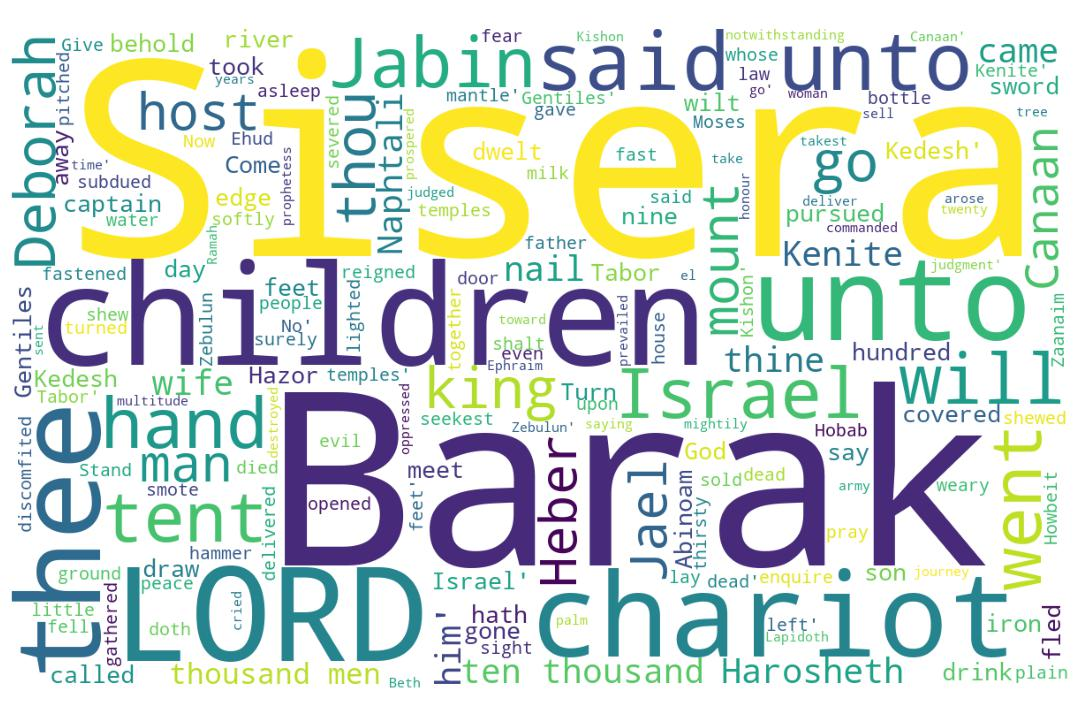
\includegraphics[width=\linewidth]{07OT-Judges/Judges4-WordCloud.jpg}
  \caption{Judges 4 Word Cloud}
  \label{fig:Judges 4 Word Cloud}
\end{figure}


\marginpar{\scriptsize \centering \fcolorbox{bone}{lime}{\textbf{YET AGAIN}}\\ (Judges 4) \begin{compactenum}[I.][8]
    \item   A New  \textbf{Chapter}  \index[scripture]{Judges!Jdg 04:01} (Jdg 4:1) 
    \item   Same  \textbf{Choices}  \index[scripture]{Judges!Jdg 04:01} (Jdg 4:1) 
    \item   The Lord's \textbf{Command}   \index[scripture]{Judges!Jdg 04:06}    (Jdg 4:6) 
    \item   The Enemy  \textbf{Captain}  \index[scripture]{Judges!Jdg 04:06} (Jdg 6:6) 
    \item   The   \textbf{Calls}  \index[scripture]{Judges!Jdg 04:06} \index[scripture]{Judges!Jdg 04:10} (Jdg 4:6, 10) 
    \item   A  \textbf{Champion}  \index[scripture]{Judges!Jdg 04:09} (Jdg 4:9) 
    \item   The  \textbf{Chariots}  \index[scripture]{Judges!Jdg 04:13} (Jdg 4:13) 
\end{compactenum}}


\footnote{\textcolor[rgb]{0.00,0.25,0.00}{\hyperlink{JudgesTOC}{Return to end of Table of Contents.}}}\footnote{\href{https://audiobible.com/bible/judges_4.html}{\textcolor[cmyk]{0.99998,1,0,0}{Judges 4 Audio}}}\textcolor[cmyk]{0.99998,1,0,0}{And the children of Israel \fcolorbox{bone}{lime}{again} did \fcolorbox{bone}{lime}{evil} in the sight of the LORD, when Ehud was dead.}
[2] \textcolor[cmyk]{0.99998,1,0,0}{And the LORD sold them into the hand of Jabin king of Canaan, that reigned in Hazor; the captain of whose host \emph{was} \fcolorbox{bone}{bone}{Sisera}, which dwelt in Harosheth of the Gentiles.}
[3] \textcolor[cmyk]{0.99998,1,0,0}{And the children of Israel cried unto the LORD: for he had nine hundred chariots of iron; and twenty years he mightily oppressed the children of Israel.}\\
\\
\P \textcolor[cmyk]{0.99998,1,0,0}{And Deborah, a prophetess, the wife of Lapidoth, she judged Israel at that time.}
[5] \textcolor[cmyk]{0.99998,1,0,0}{And she dwelt under the palm tree of Deborah between Ramah and Beth-el in mount Ephraim: and the children of Israel came up to her for judgment.}
[6] \textcolor[cmyk]{0.99998,1,0,0}{And she sent and called Barak the son of Abinoam out of Kedesh-naphtali, and said unto him, Hath not the LORD God of Israel \fcolorbox{bone}{lime}{commanded}, \emph{saying}, Go and draw toward mount Tabor, and take with thee ten thousand men of the children of Naphtali and of the children of Zebulun?}
[7] \textcolor[cmyk]{0.99998,1,0,0}{And I will draw unto thee to the river Kishon \fcolorbox{bone}{bone}{Sisera}, the captain of Jabin's army, with his chariots and his multitude; and I will deliver him into thine hand.}
[8] \textcolor[cmyk]{0.99998,1,0,0}{And Barak said unto her, If thou wilt go with me, then I will go: but if thou wilt not go with me, \emph{then} I will not go.}
[9] \textcolor[cmyk]{0.99998,1,0,0}{And she said, I will surely go with thee: notwithstanding the journey that thou takest shall not be for thine honour; for the LORD shall sell \fcolorbox{bone}{bone}{Sisera} into the hand of a woman. And \fcolorbox{bone}{lime}{Deborah} arose, and went with Barak to Kedesh.}\\
\\
\P \textcolor[cmyk]{0.99998,1,0,0}{And Barak \fcolorbox{bone}{lime}{called} Zebulun and Naphtali to Kedesh; and he went up with ten thousand men at his feet: and Deborah went up with him.}
[11] \textcolor[cmyk]{0.99998,1,0,0}{Now Heber the Kenite, \emph{which} \emph{was} of the children of Hobab the father in law of Moses, had severed himself from the Kenites, and pitched his tent unto the plain of Zaanaim, which \emph{is} by Kedesh.}
[12] \textcolor[cmyk]{0.99998,1,0,0}{And they shewed \fcolorbox{bone}{bone}{Sisera} that Barak the son of Abinoam was gone up to mount Tabor.}
[13] \textcolor[cmyk]{0.99998,1,0,0}{And \fcolorbox{bone}{bone}{Sisera} gathered together all his \fcolorbox{bone}{lime}{chariots}, \emph{even} nine hundred chariots of iron, and all the people that \emph{were} with him, from Harosheth of the Gentiles unto the river of Kishon.}\
[14] \textcolor[cmyk]{0.99998,1,0,0}{And Deborah said unto Barak, Up; for this \emph{is} the day in which the LORD hath delivered \fcolorbox{bone}{bone}{Sisera} into thine hand: is not the LORD gone out before thee? So Barak went down from mount Tabor, and ten thousand men after him.}
[15] \textcolor[cmyk]{0.99998,1,0,0}{And the LORD discomfited \fcolorbox{bone}{bone}{Sisera}, and all \emph{his} chariots, and all \emph{his} host, with the edge of the sword before Barak; so that \fcolorbox{bone}{bone}{Sisera} lighted down off \emph{his} chariot, and fled away on his feet.}
[16] \textcolor[cmyk]{0.99998,1,0,0}{But Barak pursued after the chariots, and after the host, unto Harosheth of the Gentiles: and all the host of \fcolorbox{bone}{bone}{Sisera} fell upon the edge of the sword; \emph{and} there was not a man left.}
[17] \textcolor[cmyk]{0.99998,1,0,0}{Howbeit \fcolorbox{bone}{bone}{Sisera} fled away on his feet to the tent of Jael the wife of Heber the Kenite: for \emph{there} \emph{was} peace between Jabin the king of Hazor and the house of Heber the Kenite.}\\
\\
\P \textcolor[cmyk]{0.99998,1,0,0}{And Jael went out to meet \fcolorbox{bone}{bone}{Sisera}, and said unto him, Turn in, my lord, turn in to me; fear not. And when he had turned in unto her into the tent, she covered him with a mantle.}
[19] \textcolor[cmyk]{0.99998,1,0,0}{And he said unto her, Give me, I pray thee, a little water to drink; for I am thirsty. And she opened a bottle of milk, and gave him drink, and covered him.}
[20] \textcolor[cmyk]{0.99998,1,0,0}{Again he said unto her, Stand in the door of the tent, and it shall be, when any man doth come and enquire of thee, and say, Is there any man here? that thou shalt say, No.}
[21] \textcolor[cmyk]{0.99998,1,0,0}{Then Jael Heber's wife took a nail of the tent, and took an hammer in her hand, and went softly unto him, and smote the nail into his temples, and fastened it into the ground: for he was fast asleep and weary. So he died.}
[22] \textcolor[cmyk]{0.99998,1,0,0}{And, behold, as Barak pursued \fcolorbox{bone}{bone}{Sisera}, Jael came out to meet him, and said unto him, Come, and I will shew thee the man whom thou seekest. And when he came into her \emph{tent}, behold, \fcolorbox{bone}{bone}{Sisera} lay dead, and the nail \emph{was} in his temples.}
[23] \textcolor[cmyk]{0.99998,1,0,0}{So God subdued on that day Jabin the king of Canaan before the children of Israel.}
[24] \textcolor[cmyk]{0.99998,1,0,0}{And the hand of the children of Israel prospered, and prevailed against Jabin the king of Canaan, until they had destroyed Jabin king of Canaan.}
\chapter{Judges 5}

\begin{figure}
  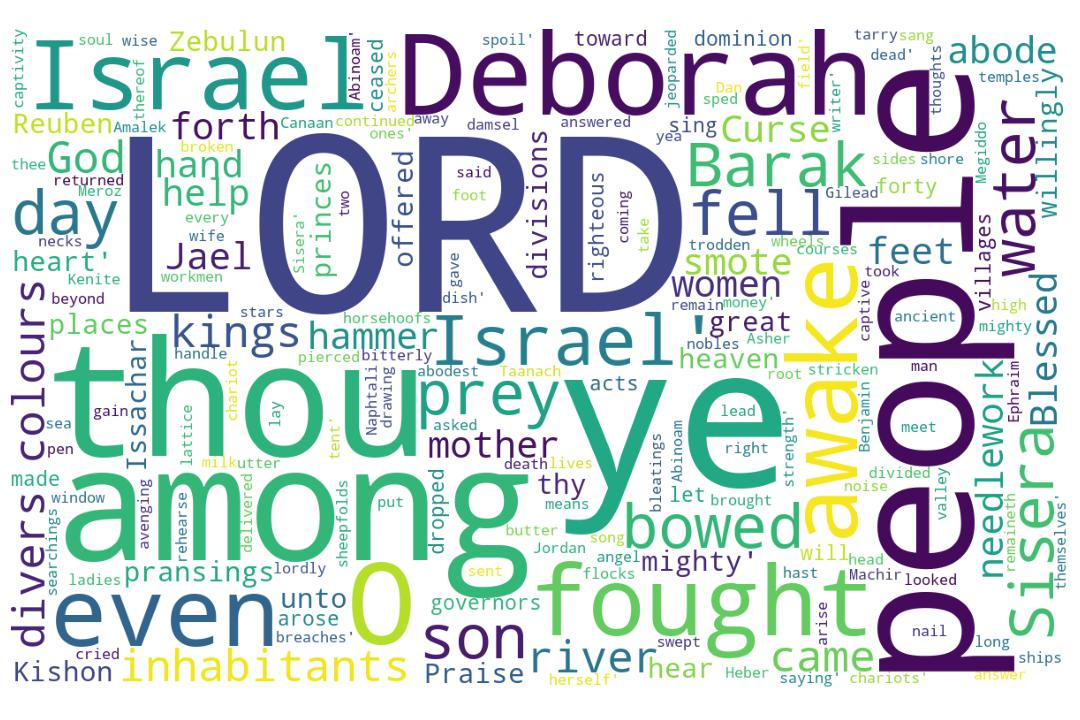
\includegraphics[width=\linewidth]{07OT-Judges/Judges5-WordCloud.jpg}
  \caption{Judges 5 Word Cloud}
  \label{fig:Judges 5 Word Cloud}
\end{figure}


\marginpar{\scriptsize \centering \fcolorbox{bone}{lime}{\textbf{A VICTORY SONG}}\\ (Judges 5) \begin{compactenum}[I.][8]
     \item   The  \textbf{March}  \index[scripture]{Judges!Jdg 05:04} (Jdg 5:4) 
    \item   The  \textbf{Mountains}  \index[scripture]{Judges!Jdg 05:05} (Jdg 5:5) 
    \item   The  \textbf{Melting}  \index[scripture]{Judges!Jdg 05:05} (Jdg 5:5) 
    \item   A  \textbf{Mother}  \index[scripture]{Judges!Jdg 05:07} (Jdg 5:7) 
    \item    \textbf{Mighty Ones}  \index[scripture]{Judges!Jdg 05:13} \index[scripture]{Judges!Jdg 05:22} \index[scripture]{Judges!Jdg 05:23} (Jdg 5:13, 22, 23) 
    \item    \textbf{Megiddo}  \index[scripture]{Judges!Jdg 05:19} (Jdg 5:19) 
    \item   The  \textbf{Dominion}  \index[scripture]{Judges!Jdg 05:13} (Jdg 5:13) 
\end{compactenum}}



\footnote{\textcolor[rgb]{0.00,0.25,0.00}{\hyperlink{JudgesTOC}{Return to end of Table of Contents.}}}\footnote{\href{https://audiobible.com/bible/judges_5.html}{\textcolor[cmyk]{0.99998,1,0,0}{Judges 5 Audio}}}\textcolor[cmyk]{0.99998,1,0,0}{Then sang Deborah and Barak the son of Abinoam on that day, saying,}
[2] \textcolor[cmyk]{0.99998,1,0,0}{Praise ye the LORD for the avenging of Israel, when the people willingly offered themselves.}
[3] \textcolor[cmyk]{0.99998,1,0,0}{Hear, O ye kings; give ear, O ye princes; I, \emph{even} I, will sing unto the LORD; I will sing \emph{praise} to the LORD God of Israel.}
[4] \textcolor[cmyk]{0.99998,1,0,0}{LORD, when thou wentest out of Seir, when thou marchedst out of the field of Edom, the earth trembled, and the heavens dropped, the clouds also dropped water.}
[5] \textcolor[cmyk]{0.99998,1,0,0}{The mountains melted from before the LORD, \emph{even} that Sinai from before the LORD God of Israel.}
[6] \textcolor[cmyk]{0.99998,1,0,0}{In the days of Shamgar the son of Anath, in the days of Jael, the highways were unoccupied, and the travellers walked through byways.}
[7] \textcolor[cmyk]{0.99998,1,0,0}{\emph{The} \emph{inhabitants} \emph{of} the villages ceased, they ceased in Israel, until that I Deborah arose, that I arose a mother in Israel.}
[8] \textcolor[cmyk]{0.99998,1,0,0}{They chose new gods; then \emph{was} war in the gates: was there a shield or spear seen among forty thousand in Israel?}
[9] \textcolor[cmyk]{0.99998,1,0,0}{My heart \emph{is} toward the governors of Israel, that offered themselves willingly among the people. Bless ye the LORD.}
[10] \textcolor[cmyk]{0.99998,1,0,0}{Speak, ye that ride on white asses, ye that sit in judgment, and walk by the way.}
[11] \textcolor[cmyk]{0.99998,1,0,0}{\emph{They} \emph{that} \emph{are} \emph{delivered} from the noise of archers in the places of drawing water, there shall they rehearse the righteous acts of the LORD, \emph{even} the righteous acts \emph{toward} \emph{the} \emph{inhabitants} of his villages in Israel: then shall the people of the LORD go down to the gates.}
[12] \textcolor[cmyk]{0.99998,1,0,0}{Awake, awake, Deborah: awake, awake, utter a song: arise, Barak, and lead thy captivity captive, thou son of Abinoam.}
[13] \textcolor[cmyk]{0.99998,1,0,0}{Then he made him that remaineth have dominion over the nobles among the people: the LORD made me have dominion over the mighty.}
[14] \textcolor[cmyk]{0.99998,1,0,0}{Out of Ephraim \emph{was} \emph{there} a root of them against Amalek; after thee, Benjamin, among thy people; out of Machir came down governors, and out of Zebulun they that handle the pen of the writer.}
[15] \textcolor[cmyk]{0.99998,1,0,0}{And the princes of Issachar \emph{were} with Deborah; even Issachar, and also Barak: he was sent on foot into the valley. For the divisions of Reuben \emph{there} \emph{were} great thoughts of heart.}
[16] \textcolor[cmyk]{0.99998,1,0,0}{Why abodest thou among the sheepfolds, to hear the bleatings of the flocks? For the divisions of Reuben \emph{there} \emph{were} great searchings of heart.}
[17] \textcolor[cmyk]{0.99998,1,0,0}{Gilead abode beyond Jordan: and why did Dan remain in ships? Asher continued on the sea shore, and abode in his breaches.}
[18] \textcolor[cmyk]{0.99998,1,0,0}{Zebulun and Naphtali \emph{were} a people \emph{that} jeoparded their lives unto the death in the high places of the field.}
[19] \textcolor[cmyk]{0.99998,1,0,0}{The kings came \emph{and} fought, then fought the kings of Canaan in Taanach by the waters of Megiddo; they took no gain of money.}
[20] \textcolor[cmyk]{0.99998,1,0,0}{They fought from heaven; the stars in their courses fought against Sisera.}
[21] \textcolor[cmyk]{0.99998,1,0,0}{The river of Kishon swept them away, that ancient river, the river Kishon. O my soul, thou hast trodden down strength.}
[22] \textcolor[cmyk]{0.99998,1,0,0}{Then were the horsehoofs broken by the means of the pransings, the pransings of their mighty ones.}
[23] \textcolor[cmyk]{0.99998,1,0,0}{Curse ye Meroz, said the angel of the LORD, curse ye bitterly the inhabitants thereof; because they came not to the help of the LORD, to the help of the LORD against the mighty.}
[24] \textcolor[cmyk]{0.99998,1,0,0}{Blessed above women shall Jael the wife of Heber the Kenite be, blessed shall she be above women in the tent.}
[25] \textcolor[cmyk]{0.99998,1,0,0}{He asked water, \emph{and} she gave \emph{him} milk; she brought forth butter in a lordly dish.}
[26] \textcolor[cmyk]{0.99998,1,0,0}{She put her hand to the nail, and her right hand to the workmen's hammer; and with the hammer she smote Sisera, she smote off his head, when she had pierced and stricken through his temples.}
[27] \textcolor[cmyk]{0.99998,1,0,0}{At her feet he bowed, he fell, he lay down: at her feet he bowed, he fell: where he bowed, there he fell down dead.}
[28] \textcolor[cmyk]{0.99998,1,0,0}{The mother of Sisera looked out at a window, and cried through the lattice, Why is his chariot \emph{so} long in coming? why tarry the wheels of his chariots?}
[29] \textcolor[cmyk]{0.99998,1,0,0}{Her wise ladies answered her, yea, she returned answer to herself,}\index[AWIP]{Her!Judges!Jdg 05:029}\index[AWIP]{wise!Judges!Jdg 05:029}\index[AWIP]{ladies!Judges!Jdg 05:029}\index[AWIP]{answered!Judges!Jdg 05:029}\index[AWIP]{her!Judges!Jdg 05:029}\index[AWIP]{yea!Judges!Jdg 05:029}\index[AWIP]{she!Judges!Jdg 05:029}\index[AWIP]{returned!Judges!Jdg 05:029}\index[AWIP]{answer!Judges!Jdg 05:029}\index[AWIP]{to!Judges!Jdg 05:029}\index[AWIP]{herself!Judges!Jdg 05:029}\index[NWIV]{11!Judges!Jdg 05:029}
[30] \textcolor[cmyk]{0.99998,1,0,0}{Have they not sped? have they \emph{not} divided the prey; to every man a damsel \emph{or} two; to Sisera a prey of divers colours, a prey of divers colours of needlework, of divers colours of needlework on both sides, \emph{meet} for the necks of \emph{them} \emph{that} \emph{take} the spoil?}
[31] \textcolor[cmyk]{0.99998,1,0,0}{So let all thine enemies perish, O LORD: but \emph{let} them that love him \emph{be} as the sun when he goeth forth in his might. And the land had rest forty years}
\chapter{Judges 6}

\begin{figure}
  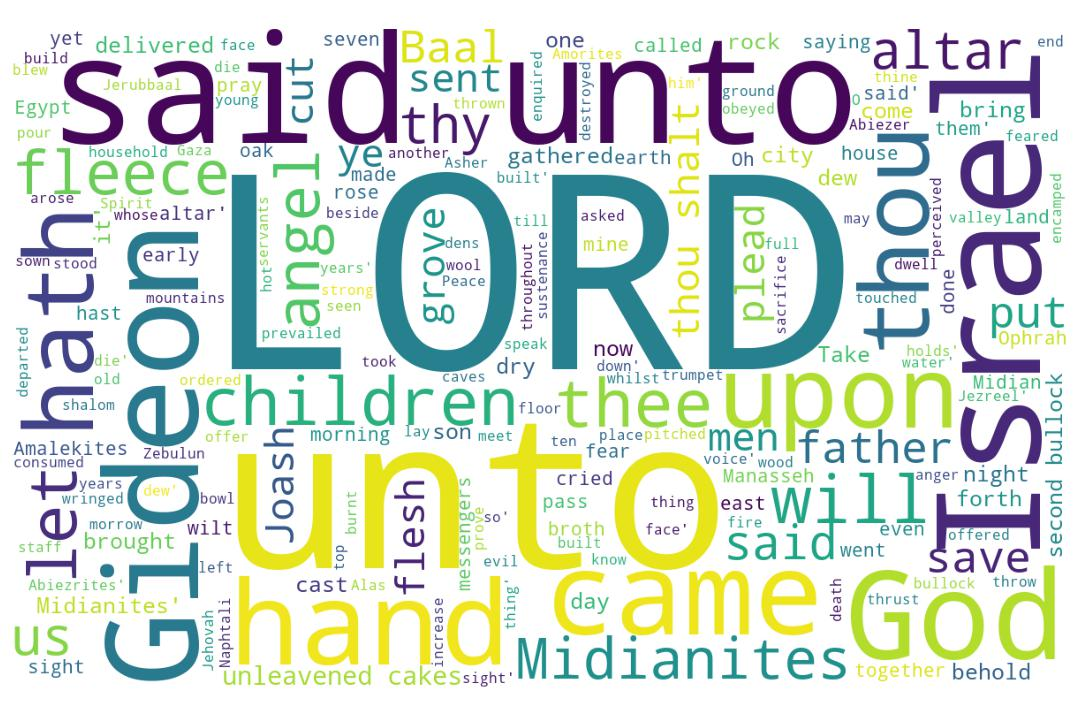
\includegraphics[width=\linewidth]{07OT-Judges/Judges6-WordCloud.jpg}
  \caption{Judges 6 Word Cloud}
  \label{fig:Judges 6 Word Cloud}
\end{figure}


\marginpar{\scriptsize \centering \fcolorbox{bone}{lime}{\textbf{GIDEON READY}}\\ (Judges 1:1-36) \begin{compactenum}[I.][8]
    \item   The  \textbf{Captivity}  \index[scripture]{Judges!Jdg 06:01} (Jdg 6:1) 
    \item   \textbf{Cave} Men \index[scripture]{Judges!Jdg 06:02} (Jdg 6:2) 
    \item   \textbf{Crops}  \index[scripture]{Judges!Jdg 06:04} (Jdg 6:4) 
    \item   The \textbf{Cry}  \index[scripture]{Judges!Jdg 06:06} (Jdg 6:6) 
    \item   Another \textbf{Champion}  \index[scripture]{Judges!Jdg 06:11} (Jdg 6:11) 
    \item   \textbf{Cakes}  \index[scripture]{Judges!Jdg 06:19--21} (Jdg 6:19--21) 
    \item   The \textbf{Conformed Ones}  \index[scripture]{Judges!Jdg 06:30} (Jdg 6:30) 
\end{compactenum}}


\footnote{\textcolor[cmyk]{0.99998,1,0,0}{\hyperlink{TOC}{Return to end of Table of Contents.}}}\footnote{\href{https://audiobible.com/bible/judges_6.html}{\textcolor[cmyk]{0.99998,1,0,0}{Judges 6 Audio}}}\textcolor[cmyk]{0.99998,1,0,0}{And the children of Israel did evil in the sight of the LORD: and the LORD delivered them into the \fcolorbox{bone}{lime}{hand of Midian} seven years.}
[2] \textcolor[cmyk]{0.99998,1,0,0}{And the hand of Midian prevailed against Israel: \emph{and} because of the Midianites the children of Israel made them the dens which \emph{are} in the mountains, and \fcolorbox{bone}{lime}{caves}, and strong holds.}
[3] \textcolor[cmyk]{0.99998,1,0,0}{And \emph{so} \fcolorbox{bone}{bone}{it} was, when Israel had sown, that the Midianites came up, and the Amalekites, and the children of the east, even they came up against them;}
[4] \textcolor[cmyk]{0.99998,1,0,0}{And they encamped against them, and destroyed the \fcolorbox{bone}{lime}{increase} of the earth, till thou come unto Gaza, and left no sustenance for Israel, neither sheep, nor ox, nor ass.}
[5] \textcolor[cmyk]{0.99998,1,0,0}{For they came up with their cattle and their tents, and they came as grasshoppers for multitude; \emph{for} both they and their camels were without number: and they entered into the land to destroy \fcolorbox{bone}{bone}{it}.}
[6] \textcolor[cmyk]{0.99998,1,0,0}{And Israel was greatly impoverished because of the Midianites; and the children of Israel \fcolorbox{bone}{lime}{cried} unto the LORD.}\\
\\
\P \textcolor[cmyk]{0.99998,1,0,0}{And \fcolorbox{bone}{bone}{it} came to pass, when the children of Israel cried unto the LORD because of the Midianites,}
[8] \textcolor[cmyk]{0.99998,1,0,0}{That the LORD sent a prophet unto the children of Israel, which said unto them, Thus saith the LORD God of Israel, I brought you up from Egypt, and brought you forth out of the house of bondage;}\
[9] \textcolor[cmyk]{0.99998,1,0,0}{And I delivered you out of the hand of the Egyptians, and out of the hand of all that oppressed you, and drave them out from before you, and gave you their land;}
[10] \textcolor[cmyk]{0.99998,1,0,0}{And I said unto you, I \emph{am} the LORD your God; fear not the gods of the Amorites, in whose land ye dwell: but ye have not obeyed my voice.}\\
\\
\P \textcolor[cmyk]{0.99998,1,0,0}{And there came an angel of the LORD, and sat under an oak which \emph{was} in Ophrah, that \emph{pertained} unto Joash the Abiezrite: and his son \fcolorbox{bone}{lime}{Gideon} threshed wheat by the winepress, to hide \emph{it} from the Midianites.}
[12] \textcolor[cmyk]{0.99998,1,0,0}{And the angel of the LORD appeared unto him, and said unto him, The LORD \emph{is} with thee, thou mighty man of valour.}
[13] \textcolor[cmyk]{0.99998,1,0,0}{And Gideon said unto him, Oh my Lord, if the LORD be with us, why then is all this befallen us? and where \emph{be} all his miracles which our fathers told us of, saying, Did not the LORD bring us up from Egypt? but now the LORD hath forsaken us, and delivered us into the hands of the Midianites.}
[14] \textcolor[cmyk]{0.99998,1,0,0}{And the LORD looked upon him, and said, Go in this thy might, and thou shalt save Israel from the hand of the Midianites: have not I sent thee?}
[15] \textcolor[cmyk]{0.99998,1,0,0}{And he said unto him, Oh my Lord, wherewith shall I save Israel? behold, my family \emph{is} poor in Manasseh, and I \emph{am} the least in my father's house.}
[16] \textcolor[cmyk]{0.99998,1,0,0}{And the LORD said unto him, Surely I will be with thee, and thou shalt smite the Midianites as one man.}
[17] \textcolor[cmyk]{0.99998,1,0,0}{And he said unto him, If now I have found grace in thy sight, then shew me a sign that thou talkest with me.}
[18] \textcolor[cmyk]{0.99998,1,0,0}{Depart not hence, I pray thee, until I come unto thee, and bring forth my present, and set \emph{it} before thee. And he said, I will tarry until thou come again.}\\
\\
\P \textcolor[cmyk]{0.99998,1,0,0}{And Gideon went in, and made ready a kid, and unleavened \fcolorbox{bone}{lime}{cakes} of an ephah of flour: the flesh he put in a basket, and he put the broth in a pot, and brought \emph{it} out unto him under the oak, and presented \emph{it}.}
[20] \textcolor[cmyk]{0.99998,1,0,0}{And the angel of God said unto him, Take the flesh and the unleavened cakes, and lay \emph{them} upon this rock, and pour out the broth. And he did so.}\\
\\
\P \textcolor[cmyk]{0.99998,1,0,0}{Then the angel of the LORD put forth the end of the staff that \emph{was} in his hand, and touched the flesh and the unleavened cakes; and there rose up fire out of the rock, and consumed the flesh and the unleavened cakes. Then the angel of the LORD departed out of his sight.}
[22] \textcolor[cmyk]{0.99998,1,0,0}{And when Gideon perceived that he \emph{was} an angel of the LORD, Gideon said, Alas, O Lord GOD! for because I have seen an angel of the LORD face to face.}
[23] \textcolor[cmyk]{0.99998,1,0,0}{And the LORD said unto him, Peace \emph{be} unto thee; fear not: thou shalt not die.}
[24] \textcolor[cmyk]{0.99998,1,0,0}{Then Gideon built an altar there unto the LORD, and called \fcolorbox{bone}{bone}{it} Jehovah-shalom: unto this day \fcolorbox{bone}{bone}{it} \emph{is} yet in Ophrah of the Abiezrites.}\\
\\
\P \textcolor[cmyk]{0.99998,1,0,0}{And \fcolorbox{bone}{bone}{it} came to pass the same night, that the LORD said unto him, Take thy father's young bullock, even the second bullock of seven years old, and throw down the altar of Baal that thy father hath, and cut down the grove that \emph{is} by \fcolorbox{bone}{bone}{it}:}
[26] \textcolor[cmyk]{0.99998,1,0,0}{And build an altar unto the LORD thy God upon the top of this rock, in the ordered place, and take the second bullock, and offer a burnt sacrifice with the wood of the grove which thou shalt cut down.}
[27] \textcolor[cmyk]{0.99998,1,0,0}{Then Gideon took ten men of his servants, and did as the LORD had said unto him: and \emph{so} \fcolorbox{bone}{bone}{it} was, because he feared his father's household, and the men of the city, that he could not do \emph{it} by day, that he did \emph{it} by night.}\\
\\
\P \textcolor[cmyk]{0.99998,1,0,0}{And when the men of the city arose early in the morning, behold, the altar of Baal was cast down, and the grove was cut down that \emph{was} by \fcolorbox{bone}{bone}{it}, and the second bullock was offered upon the altar \emph{that} \emph{was} built.}
[29] \textcolor[cmyk]{0.99998,1,0,0}{And they said one to another, Who hath done this thing? And when they enquired and asked, they said, Gideon the son of Joash hath done this thing.}
[30] \textcolor[cmyk]{0.99998,1,0,0}{Then the \fcolorbox{bone}{lime}{men of the city} said unto Joash, Bring out thy son, that he may die: because he hath cast down the altar of Baal, and because he hath cut down the grove that \emph{was} by \fcolorbox{bone}{bone}{it}.}
[31] \textcolor[cmyk]{0.99998,1,0,0}{And Joash said unto all that stood against him, Will ye plead for Baal? will ye save him? he that will plead for him, let him be put to death whilst \emph{it} \emph{is} \emph{yet} morning: if he \emph{be} a god, let him plead for himself, because \emph{one} hath cast down his altar.}
[32] \textcolor[cmyk]{0.99998,1,0,0}{Therefore on that day he called him Jerubbaal, saying, Let Baal plead against him, because he hath thrown down his altar.}\\
\\
\P \textcolor[cmyk]{0.99998,1,0,0}{Then all the Midianites and the Amalekites and the children of the east were gathered together, and went over, and pitched in the valley of Jezreel.}
[34] \textcolor[cmyk]{0.99998,1,0,0}{But the Spirit of the LORD came upon Gideon, and he blew a trumpet; and Abiezer was gathered after him.}
[35] \textcolor[cmyk]{0.99998,1,0,0}{And he sent messengers throughout all Manasseh; who also was gathered after him: and he sent messengers unto Asher, and unto Zebulun, and unto Naphtali; and they came up to meet them.}\\
\\
\P \textcolor[cmyk]{0.99998,1,0,0}{And Gideon said unto God, If thou wilt save Israel by mine hand, as thou hast said,}
[37] \textcolor[cmyk]{0.99998,1,0,0}{Behold, I will put a fleece of wool in the floor; \emph{and} if the dew be on the fleece only, and \emph{it} \emph{be} dry upon all the earth \emph{beside}, then shall I know that thou wilt save Israel by mine hand, as thou hast said.}
[38] \textcolor[cmyk]{0.99998,1,0,0}{And \fcolorbox{bone}{bone}{it} was so: for he rose up early on the morrow, and thrust the fleece together, and wringed the dew out of the fleece, a bowl full of water.}
[39] \textcolor[cmyk]{0.99998,1,0,0}{And Gideon said unto God, Let not thine anger be hot against me, and I will speak but this once: let me prove, I pray thee, but this once with the fleece; let \fcolorbox{bone}{bone}{it} now be dry only upon the fleece, and upon all the ground let there be dew.}
[40] \textcolor[cmyk]{0.99998,1,0,0}{And God did so that night: for \fcolorbox{bone}{bone}{it} was dry upon the fleece only, and there was dew on all the ground.}

\chapter{Psalm 74}

\begin{figure}
  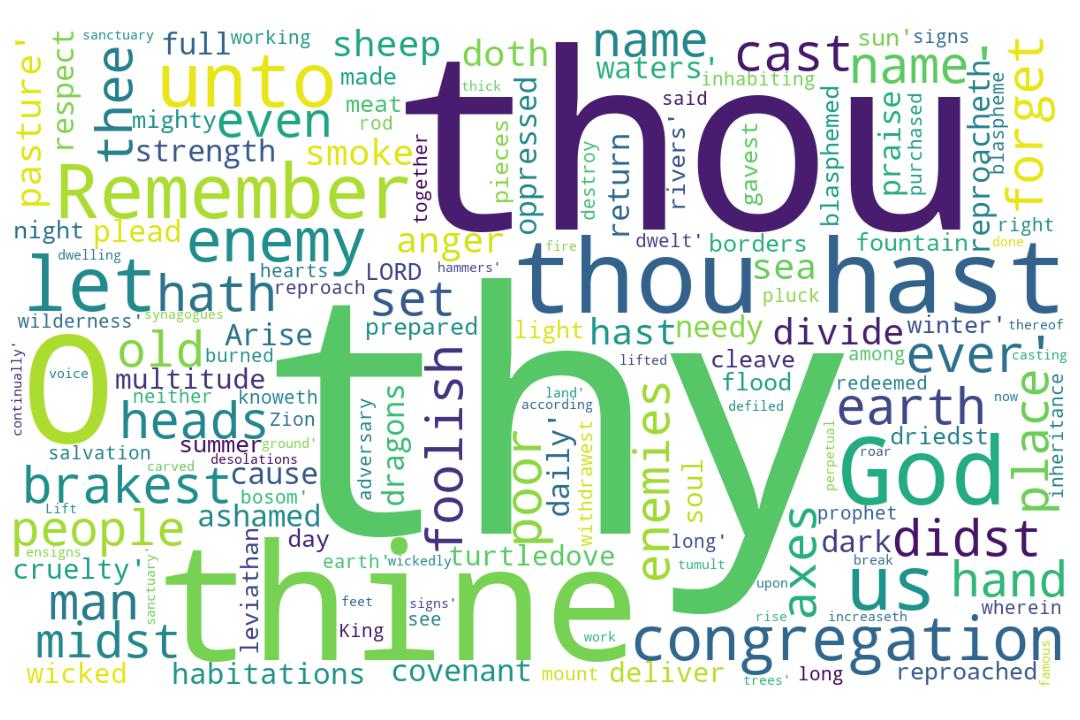
\includegraphics[width=\linewidth]{19OT-Psalms/Psalm74-WordCloud.jpg}
  \caption{Psalm 74 Word Cloud}
  \label{fig:Psalm 74 word Cloud}
\end{figure}


\marginpar{\scriptsize \centering \fcolorbox{bone}{lime}{\textbf{TIMES OF THE GENTILES OVER}}\\ (Psalm 74:1-23) \begin{compactenum}[I.][8]
    \item The \textbf{Smoke} of God's Passion \index[scripture]{Psalms!Psa 074:01}(Psa 74:1)
    \item The \textbf{Sheep} of God's Pasture \index[scripture]{Psalms!Psa 074:01}(Psa 74:1)
    \item The \textbf{Sanctuary} Polluted \index[scripture]{Psalms!Psa 074:03}(Psa 74:3)
    \item The \textbf{Signs} for the People \index[scripture]{Psalms!Psa 074:04}(Psa 74:4)
    \item God's \textbf{Strength}  \index[scripture]{Psalms!Psa 074:13}(Psa 74:13)
   \item \textbf{Supply}  Provided \index[scripture]{Psalms!Psa 074:14}(Psa 74:14)
   \item \textbf{Souls}  Protected \index[scripture]{Psalms!Psa 074:19}(Psa 74:19)
\end{compactenum}}
    



\footnote{\textcolor[cmyk]{0.99998,1,0,0}{\hyperlink{TOC}{Return to end of Table of Contents.}}}\footnote{\href{https://audiobible.com/bible/psalms_74.html}{\textcolor[cmyk]{0.99998,1,0,0}{Psalm 74 Audio}}}\textcolor[cmyk]{0.99998,1,0,0}{Maschil of Asaph}\\
\\
\textcolor[cmyk]{0.99998,1,0,0}{O God, why hast thou cast \emph{us} off for ever? \emph{why} doth thine anger \fcolorbox{bone}{lime}{smoke} against the \fcolorbox{bone}{lime}{sheep} of thy pasture?}\footnote{\textbf{Lamentations 5:20-22} - Wherefore dost thou forget us for ever, and forsake us so long time? [21] Turn thou us unto thee, O LORD, and we shall be turned; renew our days as of old. [22] But thou hast utterly rejected us; thou art very wroth against us.}\footnote{\textbf{Joel 2:32} - And it shall come to pass, that whosoever shall call on the name of the LORD shall be delivered: for in mount Zion and in Jerusalem shall be deliverance, as the LORD hath said, and in the remnant whom the LORD shall call.}\footnote{\textbf{Romans 11:2} - God hath not cast away his people which he foreknew. Wot ye not what the scripture saith of Elias? how he maketh intercession to God against Israel, saying,}\footnote{\textbf{Romans 11:26} - And so all Israel shall be saved: as it is written, There shall come out of Sion the Deliverer, and shall turn away ungodliness from Jacob:}
[2] \textcolor[cmyk]{0.99998,1,0,0}{Remember thy congregation, \emph{which} thou hast purchased of old; the rod of thine inheritance, \emph{which} thou hast redeemed; this mount Zion, wherein thou hast dwelt.}
[3] \textcolor[cmyk]{0.99998,1,0,0}{Lift up thy feet unto the perpetual desolations; \emph{even} all \emph{that} the enemy hath done wickedly in the \fcolorbox{bone}{lime}{sanctuary}.}\footnote{\textbf{Isaiah 63:18} - The people of thy holiness have possessed it but a little while: our adversaries have trodden down thy sanctuary.}\footnote{\textbf{Jeremiah 25:9, 12} - Behold, I will send and take all the families of the north, saith the LORD, and Nebuchadrezzar the king of Babylon, my servant, and will bring them against this land, and against the inhabitants thereof, and against all these nations round about, and will utterly destroy them, and make them an astonishment, and an hissing, and perpetual desolations. [12] And it shall come to pass, when seventy years are accomplished, that I will punish the king of Babylon, and that nation, saith the LORD, for their iniquity, and the land of the Chaldeans, and will make it perpetual desolations.}\footnote{\textbf{Ezekiel 35:9} - I will make thee perpetual desolations, and thy cities shall not return: and ye shall know that I am the LORD.}
[4] \textcolor[cmyk]{0.99998,1,0,0}{Thine enemies roar in the midst of thy \fcolorbox{bone}{MYGOLD}{congregations}; they set up their ensigns \emph{for} \fcolorbox{bone}{lime}{signs}.}
[5] \textcolor[cmyk]{0.99998,1,0,0}{\emph{A} \emph{man} was famous according as he had lifted up axes upon the thick trees.}
[6] \textcolor[cmyk]{0.99998,1,0,0}{But now they break down the carved work thereof at once with axes and hammers.}
[7] \textcolor[cmyk]{0.99998,1,0,0}{They have cast fire into thy sanctuary, they have defiled \emph{by} \emph{casting} \emph{down} the dwelling place of thy name to the ground.}
[8] \textcolor[cmyk]{0.99998,1,0,0}{They said in their hearts, Let us destroy them together: they have burned up all the synagogues of God in the land.}
[9] \textcolor[cmyk]{0.99998,1,0,0}{We see not our signs: \emph{there} \emph{is} no more any prophet: neither \emph{is} \emph{there} among us any that knoweth how long.}
[10] \textcolor[cmyk]{0.99998,1,0,0}{O God, how long shall the adversary reproach? shall the enemy blaspheme thy name for ever?}
[11] \textcolor[cmyk]{0.99998,1,0,0}{Why withdrawest thou thy hand, even thy right hand? pluck \emph{it} out of thy bosom.}
[12] \textcolor[cmyk]{0.99998,1,0,0}{For God \emph{is} my King of old, working salvation in the midst of the earth.}
[13] \textcolor[cmyk]{0.99998,1,0,0}{Thou didst divide the sea by thy \fcolorbox{bone}{lime}{strength}: thou brakest the heads of the dragons in the waters.}
[14] \textcolor[cmyk]{0.99998,1,0,0}{Thou brakest the heads of leviathan in pieces, \emph{and} gavest him \emph{to} \emph{be} \fcolorbox{bone}{lime}{meat} to the people inhabiting the wilderness.}
[15] \textcolor[cmyk]{0.99998,1,0,0}{Thou didst cleave the fountain and the flood: thou driedst up mighty rivers.}
[16] \textcolor[cmyk]{0.99998,1,0,0}{The day \emph{is} thine, the night also \emph{is} thine: thou hast prepared the light and the sun.}
[17] \textcolor[cmyk]{0.99998,1,0,0}{Thou hast set all the borders of the earth: thou hast made summer and winter.}
[18] \textcolor[cmyk]{0.99998,1,0,0}{Remember this, \emph{that} the enemy hath reproached, O LORD, and \emph{that} the foolish people have blasphemed thy name.}
[19] \textcolor[cmyk]{0.99998,1,0,0}{O deliver not the \fcolorbox{bone}{lime}{soul} of thy turtledove unto the multitude \emph{of} \emph{the} \emph{wicked}: forget not the congregation of thy poor for ever.}
[20] \textcolor[cmyk]{0.99998,1,0,0}{Have respect unto the covenant: for the dark places of the earth are full of the habitations of cruelty.}
[21] \textcolor[cmyk]{0.99998,1,0,0}{O let not the oppressed return ashamed: let the poor and needy praise thy name.}
[22] \textcolor[cmyk]{0.99998,1,0,0}{Arise, O God, plead thine own cause: remember how the foolish man reproacheth thee daily.}
[23] \textcolor[cmyk]{0.99998,1,0,0}{Forget not the voice of thine enemies: the tumult of those that rise up against thee increaseth continually.}





\chapter{Proverb 15}\marginpar{\scriptsize \centering \fcolorbox{bone}{lime}{\textbf{RIGHTEOUS LIPS}}\\ (Proverbs 15:1-33) \begin{compactenum}[I.][8]
    \item \textbf{Turn Away Wrath}  \index[scripture]{Proverbs!Pro 15:01}(Pro 15:1)
    \item \textbf{Dispense Knowledge} \index[scripture]{Proverbs!Pro 15:02, 07}(Pro 15:2, 7)
    \item \textbf{Are Wholesome} \index[scripture]{Proverbs!Pro 15:04}(Pro 15:4)
    \item \textbf{Offer counsel} \index[scripture]{Proverbs!Pro 15:22}(Pro 15:22)
    \item \textbf{Speak in Due Season} \index[scripture]{Proverbs!Pro 15:23}(Pro 15:23)
    \item \textbf{Are Pure and Pleasant} \index[scripture]{Proverbs!Pro 15:26}(Pro 15:26)
    \item \textbf{Answer Slowly} \index[scripture]{Proverbs!Pro 15:28}(Pro 15:28) -- some answers are not easy
\end{compactenum}}

\marginpar{\scriptsize \centering \fcolorbox{bone}{yellow}{\textbf{RESPONDING TO CORRECTION}}\\ (Proverbs 15:1-33) \begin{compactenum}[I.][8]
    \item \textbf{Wrath}  \index[scripture]{Proverbs!Pro 15:01} 
                                      \index[scripture]{Proverbs!Pro 15:18} 
                                      (Pro 15:1, 18)
    \item \textbf{Reproof}  \index[scripture]{Proverbs!Pro 15:05} 
                                      \index[scripture]{Proverbs!Pro 15:10} 
                                      \index[scripture]{Proverbs!Pro 15:12} 
                                      \index[scripture]{Proverbs!Pro 15:31} 
                                      \index[scripture]{Proverbs!Pro 15:32}  (Pro 15:5, 10, 12, 31, 32)
    \item God's \textbf{Reconnaissance}  \index[scripture]{Proverbs!Pro 15:03}  (Pro 15:3)
    \item \textbf{Regard}  \index[scripture]{Proverbs!Pro 15:05}  (Pro 15:5)
    \item \textbf{Righteousness}  \index[scripture]{Proverbs!Pro 15:06} \index[scripture]{Proverbs!Pro 15:09} \index[scripture]{Proverbs!Pro 15:19} \index[scripture]{Proverbs!Pro 15:28} 
    \index[scripture]{Proverbs!Pro 15:29}  (Pro 15:6, 9, 19, 28, 29)
    \item \textbf{Refusal}  \index[scripture]{Proverbs!Pro 15:32}  (Pro 15:32)
    \item \textbf{Receiving}  \index[scripture]{Proverbs!Pro 15:32}  (Pro 15:32)
\end{compactenum}}
    
\footnote{\textcolor[cmyk]{0.99998,1,0,0}{\hyperlink{TOC}{Return to end of Table of Contents.}}}\footnote{\href{https://audiobible.com/bible/proverbs_15.html}{\textcolor[cmyk]{0.99998,1,0,0}{Proverbs Audio}}}\textcolor[cmyk]{0.99998,1,0,0}{A soft answer \fcolorbox{bone}{lime}{turneth away wrath}: but grievous words stir up anger.}
[2] \textcolor[cmyk]{0.99998,1,0,0}{The tongue of the wise \fcolorbox{bone}{lime}{useth knowledge} aright: but the mouth of fools poureth out foolishness.}
[3] \textcolor[cmyk]{0.99998,1,0,0}{The eyes of the LORD \emph{are} in every place, beholding the evil and the good.}
[4] \textcolor[cmyk]{0.99998,1,0,0}{\fcolorbox{bone}{lime}{A wholesome tongue} \emph{is} a tree of life: but perverseness therein \emph{is} a breach in the spirit.}
[5] \textcolor[cmyk]{0.99998,1,0,0}{A fool despiseth his father's instruction: but he \fcolorbox{bone}{bone}{that} regardeth reproof is prudent.}
[6] \textcolor[cmyk]{0.99998,1,0,0}{In the house of the righteous \emph{is} much treasure: but in the revenues of the wicked is trouble.}
[7] \textcolor[cmyk]{0.99998,1,0,0}{The lips of the wise \fcolorbox{bone}{lime}{disperse knowledge}: but the heart of the foolish \emph{doeth} not so.}
[8] \textcolor[cmyk]{0.99998,1,0,0}{The sacrifice of the wicked \emph{is} an abomination to the LORD: but the prayer of the upright \emph{is} his delight.}
[9] \textcolor[cmyk]{0.99998,1,0,0}{The way of the wicked \emph{is} an abomination unto the LORD: but he loveth him \fcolorbox{bone}{bone}{that} followeth after righteousness.}
[10] \textcolor[cmyk]{0.99998,1,0,0}{Correction \emph{is} grievous unto him \fcolorbox{bone}{bone}{that} forsaketh the way: \emph{and} he \fcolorbox{bone}{bone}{that} hateth reproof shall die.}\footnote{\textbf{Jeremiah 2:30} - In vain have I smitten your children; they received no correction: your own sword hath devoured your prophets, like a destroying lion.}\footnote{\textbf{Jeremiah 5:3} - O LORD, are not thine eyes upon the truth? thou hast stricken them, but they have not grieved; thou hast consumed them, but they have refused to receive correction: they have made their faces harder than a rock; they have refused to return.}\footnote{\textbf{Jeremiah 7:28} - But thou shalt say unto them, This is a nation that obeyeth not the voice of the LORD their God, nor receiveth correction: truth is perished, and is cut off from their mouth.}\footnote{\textbf{Zephaniah 3:2} - She obeyed not the voice; she received not correction; she trusted not in the LORD; she drew not near to her God.}\footnote{\textbf{2 Timothy 3:16} - All scripture is given by inspiration of God, and is profitable for doctrine, for reproof, for correction, for instruction in righteousness:}
[11] \textcolor[cmyk]{0.99998,1,0,0}{Hell and destruction \emph{are} before the LORD: how much more then the hearts of the children of men?}
[12] \textcolor[cmyk]{0.99998,1,0,0}{A scorner loveth not one \fcolorbox{bone}{bone}{that} reproveth him: neither will he go unto the wise.}
[13] \textcolor[cmyk]{0.99998,1,0,0}{A merry heart maketh a cheerful countenance: but by sorrow of the heart the spirit is broken.}
[14] \textcolor[cmyk]{0.99998,1,0,0}{The heart of him \fcolorbox{bone}{bone}{that} hath understanding seeketh knowledge: but the mouth of fools feedeth on foolishness.}
[15] \textcolor[cmyk]{0.99998,1,0,0}{All the days of the afflicted \emph{are} evil: but he \fcolorbox{bone}{bone}{that} is of a merry heart \emph{hath} a continual feast.}
[16] \textcolor[cmyk]{0.99998,1,0,0}{Better \emph{is} little with the fear of the LORD than great treasure and trouble therewith.}
[17] \textcolor[cmyk]{0.99998,1,0,0}{Better \emph{is} a dinner of herbs where love is, than a stalled ox and hatred therewith.}
[18] \textcolor[cmyk]{0.99998,1,0,0}{A wrathful man stirreth up strife: but \emph{he} \emph{that} \emph{is} slow to anger appeaseth strife.}
[19] \textcolor[cmyk]{0.99998,1,0,0}{The way of the slothful \emph{man} \emph{is} as an hedge of thorns: but the way of the righteous \emph{is} made plain.}
[20] \textcolor[cmyk]{0.99998,1,0,0}{A wise son maketh a glad father: but a foolish man despiseth his mother.}
[21] \textcolor[cmyk]{0.99998,1,0,0}{Folly \emph{is} joy to \emph{him} \emph{that} \emph{is} destitute of wisdom: but a man of understanding walketh uprightly.}
[22] \textcolor[cmyk]{0.99998,1,0,0}{Without \fcolorbox{bone}{lime}{counsel} purposes are disappointed: but in the multitude of \fcolorbox{bone}{lime}{counsellors} they are established.}
[23] \textcolor[cmyk]{0.99998,1,0,0}{A man hath joy by the answer of his mouth: and a word \emph{spoken} \fcolorbox{bone}{lime}{in due season}, how good \emph{is} \emph{it}!}
[24] \textcolor[cmyk]{0.99998,1,0,0}{The way of life \emph{is} above to the wise, \fcolorbox{bone}{bone}{that} he may depart from hell beneath.}
[25] \textcolor[cmyk]{0.99998,1,0,0}{The LORD will destroy the house of the proud: but he will establish the border of the widow.}
[26] \textcolor[cmyk]{0.99998,1,0,0}{The thoughts of the wicked \emph{are} an abomination to the LORD: but \emph{the} \emph{words} of the pure \emph{are} \fcolorbox{bone}{lime}{pleasant words}.}
[27] \textcolor[cmyk]{0.99998,1,0,0}{He \fcolorbox{bone}{bone}{that} is greedy of gain troubleth his own house; but he \fcolorbox{bone}{bone}{that} hateth gifts shall live.}
[28] \textcolor[cmyk]{0.99998,1,0,0}{The heart of the righteous \fcolorbox{bone}{lime}{studieth to answer}: but the mouth of the wicked poureth out evil things.}
[29] \textcolor[cmyk]{0.99998,1,0,0}{The LORD \emph{is} far from the wicked: but he heareth the prayer of the righteous.}
[30] \textcolor[cmyk]{0.99998,1,0,0}{The light of the eyes rejoiceth the heart: \emph{and} a good report maketh the bones fat.}
[31] \textcolor[cmyk]{0.99998,1,0,0}{The ear \fcolorbox{bone}{bone}{that} heareth the reproof of life abideth among the wise.}
[32] \textcolor[cmyk]{0.99998,1,0,0}{He \fcolorbox{bone}{bone}{that} refuseth instruction despiseth his own soul: but he \fcolorbox{bone}{bone}{that} heareth reproof getteth understanding.}
[33] \textcolor[cmyk]{0.99998,1,0,0}{The fear of the LORD \emph{is} the instruction of wisdom; and before honour \emph{is} humility.}




\end{document}

